\section{Results}

We consider a globally isothermal disk, $c_s=\mathrm{const.}$, by
setting $q=0$ in the equation of state (Eq. \ref{eos}), and a flat
mid-plane gas density, $\rhog(0) = \mathrm{const.}$, so there is no
global radial pressure gradient at the disk midplane. This setup
eliminates classic vertical shear instability and streaming
instabilities. The stopping time is
prescribed as 
\begin{align}
  \tstop = t_\mathrm{s0}\frac{\rho(z=0)}{\rho(z)}. 
\end{align}

As an example, we set the midplane dust-to-gas ratio 
$\tepsilon_0=0.02$, dust scale-height $H_\mathrm{d}=0.6\Hgas$, and
stopping time $t_\mathrm{s0}\OmK=0.02$. We consider modes with radial
wavenumber $k_x\Hdust=2\pi$. The vertical domain size is set to  
$\zmax=2\Hgas$. The aspect-ratio of the gas layer is
$h_\mathrm{g}=0.05$. 

We use a pseudo-spectral method to solve  
Eq. \ref{lin_mass}---\ref{lin_energy} as a generalized eigenvalue
problem with $N=513$ grid points. Fig. \ref{eigen_map}   
shows a map of the eigenvalues in the $(\omega, s)$ plane. Note that
we restrict attention to modes with $|\sigma|\leq \OmK$. 
Eigenvalues on the `Y' branch should not be trusted. The 
high growth-rate modes are associated with disturbances concentrated
at the domain boundaries. Modes with $\omega\simeq 0$, i.e. purely
growing modes, are likely spurious because we generally expect
eigenvalues to be complex (see the integral relation in Appendix
\ref{var_prin}).  

\begin{figure}
  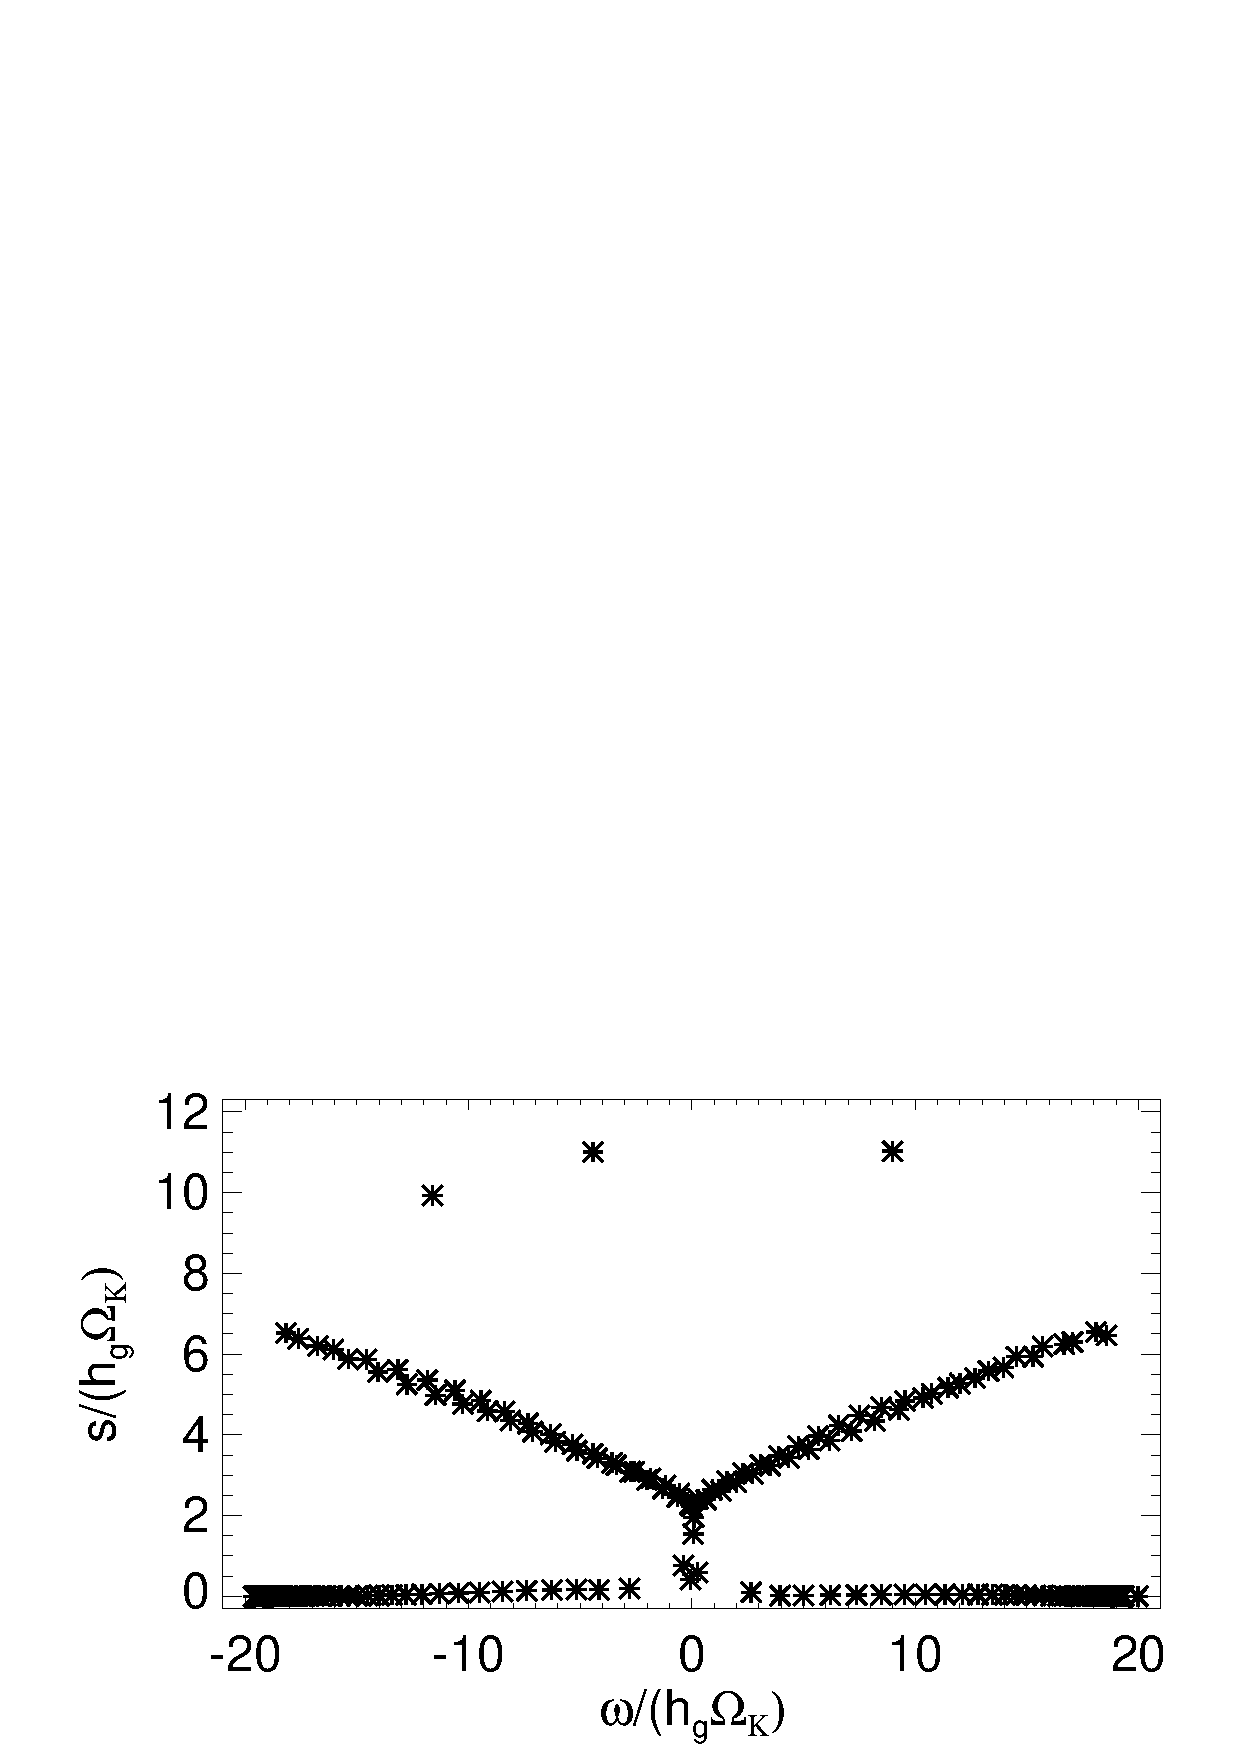
\includegraphics[width=\linewidth]{figures/eigenvalues}
  \caption{Eigenvalues found for the fiducial isothermal dusty
    problem. 
  \label{eigen_map}} 
\end{figure}

We thus consider the slower-growing modes near the horizontal
axis. Fig. \ref{eigen_vec} show example eigenfunctions for a case with
frequency $(\omega,s)=(-2.79,0.20)\hgas\OmK$. 


In Fig. \ref{eigen_2d}
we visualize this mode in the $(x,z)$ plane: colors show the
perturbation to the dust-fraction ($\dd\epsilon$), while vectors show
the perturbed meridional momenta. This mode has a growth
timescale of $\simeq 16$ orbits. This mode is unlikely driven by
vertical shear: the maximum vertical 
shear rate, $\mathrm{max}\left|r\p_z\Omega\right|\simeq10^{-2}\hgas\OmK$,
is much smaller than the mode growth rate $s\simeq 0.2\hgas\OmK$. 

\begin{figure}
  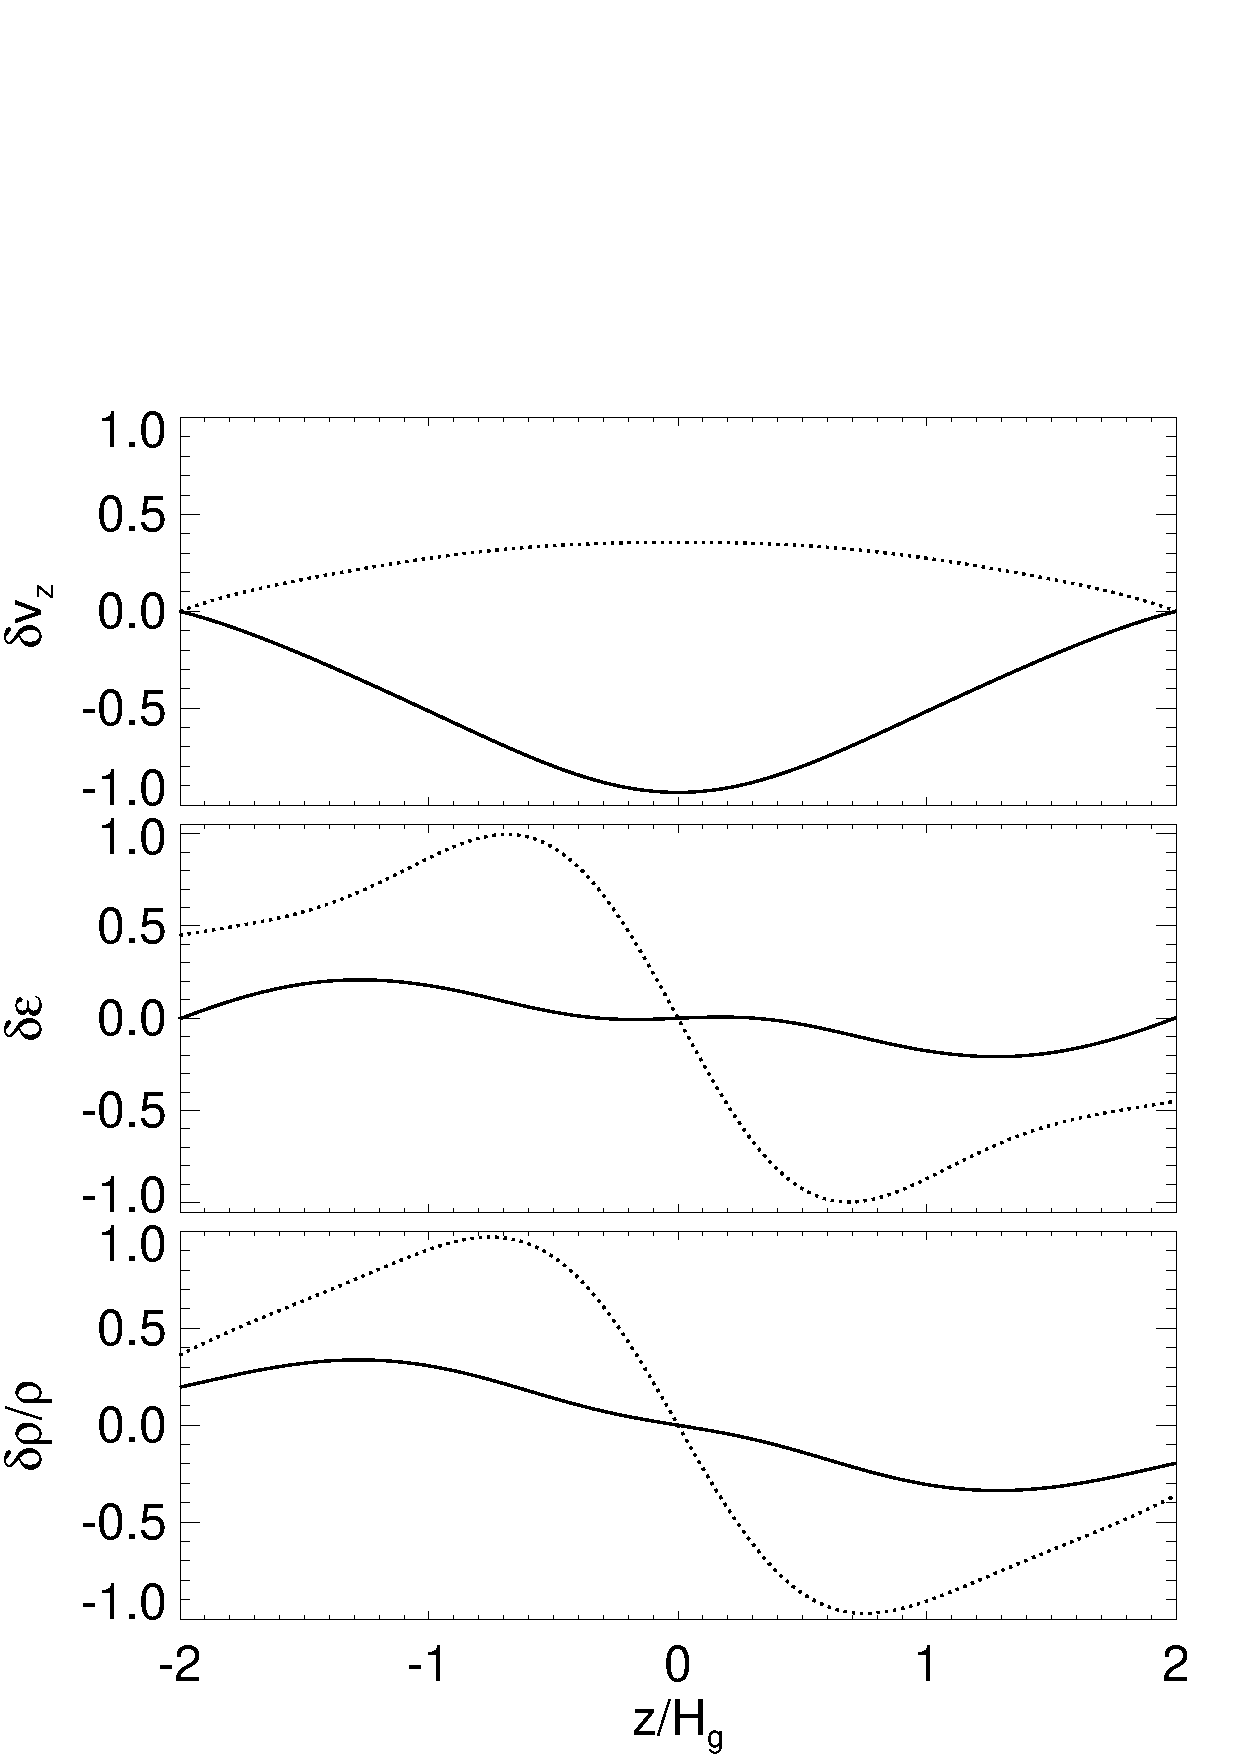
\includegraphics[width=\linewidth]{figures/eigenvec}
  \caption{Example eigenfunctions from the fiducial case. 
    \label{eigen_vec}} 
\end{figure}

\begin{figure}
  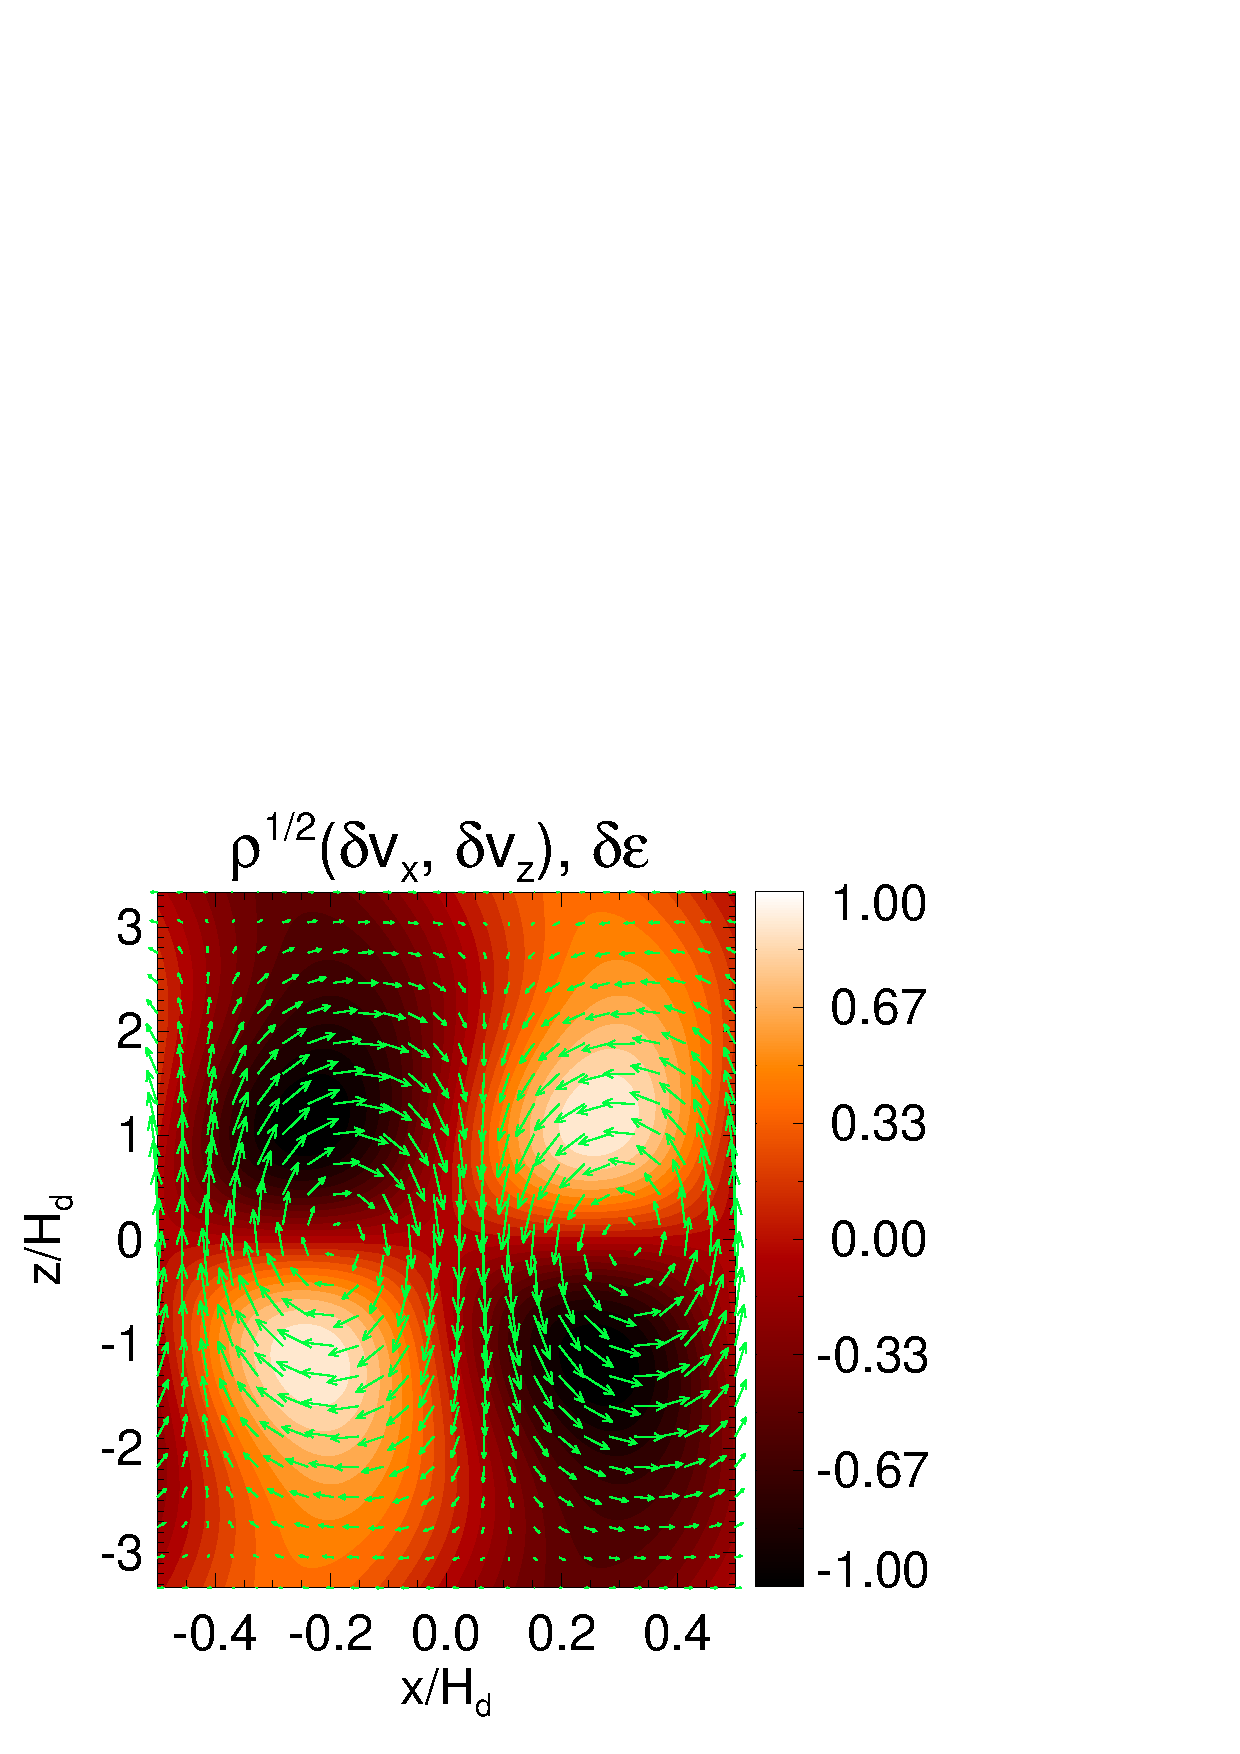
\includegraphics[width=\linewidth]{figures/result2d}
  \caption{Example eigenvectors from the fiducial case. The eigenvalue
    is $(\omega,s)=(-2.79,0.20)\hgas\OmK$.  
    \label{eigen_2d}} 
\end{figure}
